\documentclass[12pt,letterpaper]{article}

% just for the example
\usepackage{lipsum}
% Set margins to 1.5in
\usepackage[margin=1.5in]{geometry}

% for graphics
\usepackage{graphicx}
\graphicspath{{./figures/p3/}}

% for crimson text
\usepackage{crimson}
\usepackage[T1]{fontenc}

% setup parameter indentation
\setlength{\parindent}{0pt}
\setlength{\parskip}{6pt}

% for 1.15 spacing between text
\renewcommand{\baselinestretch}{1.15}

% For defining spacing between headers
\usepackage{titlesec}
% Level 1
\titleformat{\section}
  {\normalfont\fontsize{18}{0}\bfseries}{\thesection}{1em}{}
% Level 2
\titleformat{\subsection}
  {\normalfont\fontsize{14}{0}\bfseries}{\thesection}{1em}{}
% Level 3
\titleformat{\subsubsection}
  {\normalfont\fontsize{12}{0}\bfseries}{\thesection}{1em}{}
% Level 4
\titleformat{\paragraph}
  {\normalfont\fontsize{12}{0}\bfseries\itshape}{\theparagraph}{1em}{}
% Level 5
\titleformat{\subparagraph}
  {\normalfont\fontsize{12}{0}\itshape}{\theparagraph}{1em}{}
% Level 6
\makeatletter
\newcounter{subsubparagraph}[subparagraph]
\renewcommand\thesubsubparagraph{%
  \thesubparagraph.\@arabic\c@subsubparagraph}
\newcommand\subsubparagraph{%
  \@startsection{subsubparagraph}    % counter
    {6}                              % level
    {\parindent}                     % indent
    {12pt} % beforeskip
    {6pt}                           % afterskip
    {\normalfont\fontsize{12}{0}}}
\newcommand\l@subsubparagraph{\@dottedtocline{6}{10em}{5em}}
\newcommand{\subsubparagraphmark}[1]{}
\makeatother
\titlespacing*{\section}{0pt}{12pt}{6pt}
\titlespacing*{\subsection}{0pt}{12pt}{6pt}
\titlespacing*{\subsubsection}{0pt}{12pt}{6pt}
\titlespacing*{\paragraph}{0pt}{12pt}{6pt}
\titlespacing*{\subparagraph}{0pt}{12pt}{6pt}
\titlespacing*{\subsubparagraph}{0pt}{12pt}{6pt}

% Set caption to correct size and location
\usepackage[tableposition=top, figureposition=bottom, font=footnotesize, labelfont=bf]{caption}

% set page number location
\usepackage{fancyhdr}
\fancyhf{} % clear all header and footers
\renewcommand{\headrulewidth}{0pt} % remove the header rule
\rhead{\thepage}
\pagestyle{fancy}

% Overwrite Title
\makeatletter
\renewcommand{\maketitle}{\bgroup
   \begin{center}
   \textbf{{\fontsize{18pt}{20}\selectfont \@title}}\\
   \vspace{10pt}
   {\fontsize{12pt}{0}\selectfont \@author} 
   \end{center}
}
\makeatother

% Used for Tables and Figures
\usepackage{float}

% For using lists
\usepackage{enumitem}

% For using APA Citation format
\usepackage{apacite}

% Custom Quote
\newenvironment{myquote}[1]%
  {\list{}{\leftmargin=#1\rightmargin=#1}\item[]}%
  {\endlist}
  
% Create Abstract 
\renewenvironment{abstract}
{\vspace*{-.5in}\fontsize{12pt}{12}\begin{myquote}{.5in}
\noindent \par{\bfseries \abstractname.}}
{\medskip\noindent
\end{myquote}
}

\begin{document}

% Set Title, Author, and email
\title{Assignment P3}
\author{Snejana Shegheva \\ sshegheva3@gatech.edu}

\maketitle
\thispagestyle{fancy}

\subsection*{Question 1 - Design Principles and Heuristics}

\subsection*{Question 2 - Constraint, Mappings and Affordances Principles}

Although, not entirely an activity of my everyday life, I used to regularly participate in an adrenaline-raising practice of flying trapeze. For safety reasons, all students must wear belt harness. When on the platform, safety lines are attached to the belt so that a trained professional can reduce the impact of wrong falling. Figure~\ref{fig::1} demonstrates attaching a carabiner (that holds safety lines) to a belt in two ways: \textit{overhook} vs \textit{underhook}\footnote{The terms \textit{overhook} vs. \textit{underhook} in this context have nothing to do with wrestling}. The preferred way is to use \textit{overhook} position that greatly simplifies the process of detachment. Although the \textit{underhook} position is not wrong, it makes it very inconvenient for your wrists to twist the lock to open and release. It is very \textbf{easy} to hook the carabiners from savety lines to the belt harness in the sub-optimal way because there is nothing to prevent you from hooking it in either direction (and both do their job of protecting you from a fall). The \textbf{penalty} here comes \textit{after} completing the jump where you have to release the safety lines from both your sides. It takes a lot of wiggling the carabiners around to put them back in the position where it is possible to unlock them safely for subsequent transfer back to the person on the board.   

\begin{figure}[h]
\centering
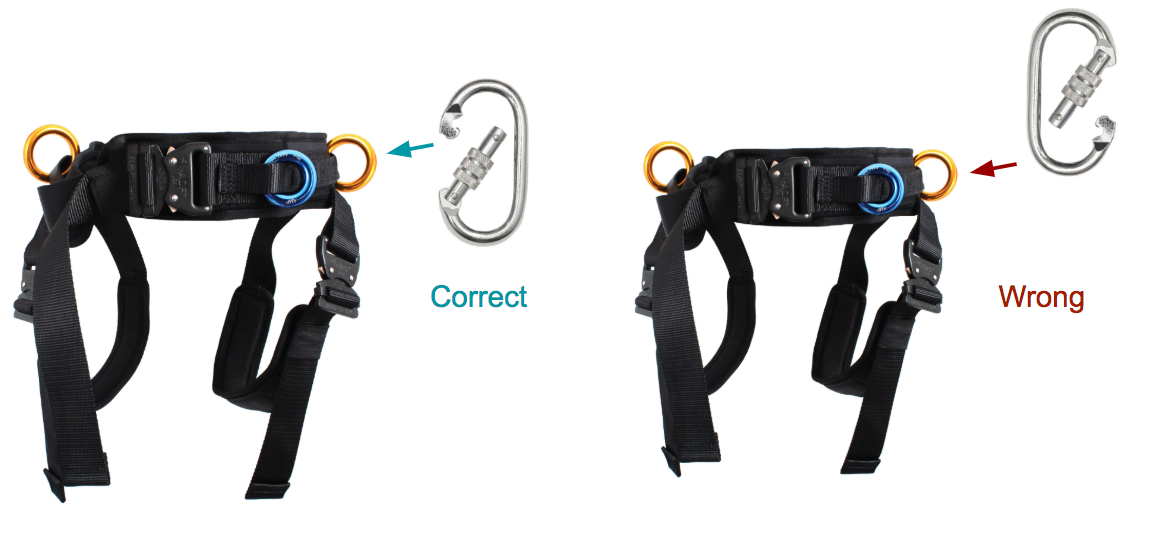
\includegraphics[width=3in,scale=.5]{figures/p3/flying_trapeze.png}
\caption{Demonstration of two ways to attach a carabiner to a belt. Left: preferred. Right: Inconvenient (especially for detaching using one hand.)}
\label{fig::1}
\end{figure}

\subsubsection*{Constraints}
One clue for limiting the wrong action is to modify the ring on the belt that constrains you from passing the hook unless it is a specific position. For example, changing the thickness of the rings in different areas can guide the proper clasping position. Alternatively, the hook on the carabiner itself can have a more intricate shape that forces you to angle it in a certain way.

\subsubsection*{Mappings}
Don Norman defines a  \textit{mappings} design principle in terms of relationship a control and resulting function\cite{norman2013design}. The result of a carabiner locking depends on how the person originally holds it. Therefore, a mapping principle suggests to add visual clues for desired alignment between the hand and the carabiner. Similarly to how some shipping packages are labeled with an arrow pointing up, the surface of the carabiner can be engraved with an arrow to hint on the direction of hold.    

\subsubsection*{Affordances}
A strong relative to mapping principle is \textit{affordance} principle that determines the interaction method between the agent and the interface \cite{norman2013design}. To improve the carabiner interface, its shape can be mapped to the shape of the palm. When we clasp our hands, it is more natural the grip to be wider closer to the thumb, and more narrow towards the pinkie. If the carabiner for flying trapeze can resemble a \textit{pear} shape, it would be more intuitive to grasp the carabiner in a certain way that it more likely for you to hook it from a right angle. The shape in this case affords a proper handle \textit{before} the carabiner is attached.


\subsection*{Question 3 - Slips, Mistakes and Errors}
Yousican is an innovate application that allows students to learn how to play piano, guitar and other musical instruments\cite{eli2017yousician}. It is a fun game that involves following step-by-step tutorials, exercises and play-alongs. At the core of learning to play a musical instrument is a lot of practice, and slips and mistakes are unavoidable part of the experience. Figure~\ref{fig::2} shows an example of a screen that user interacts with.

\begin{figure}[h]
\centering
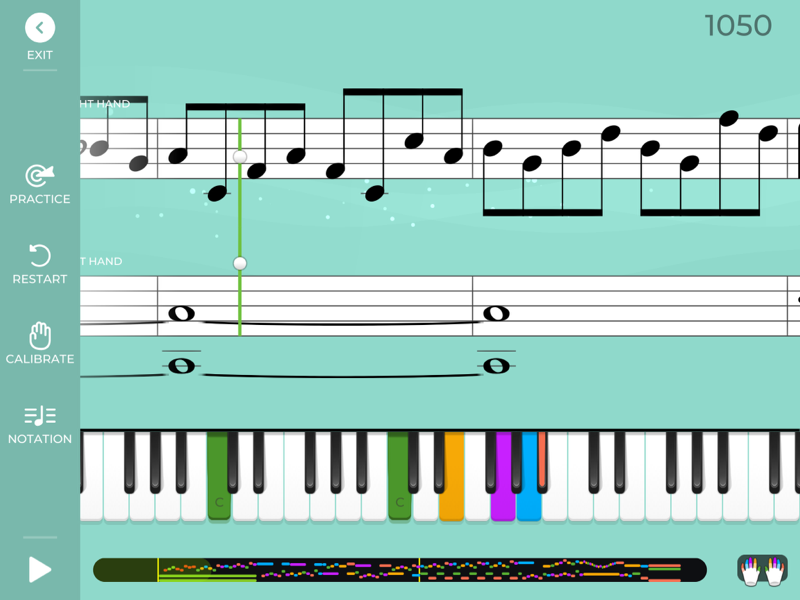
\includegraphics[width=3in,scale=.6]{figures/p3/yousician.png}
\caption{A screenshot from Yousician App that teachers the user to play piano}
\label{fig::2}
\end{figure}

\subsubsection*{Slips}
When a user follows along by playing the given music score, they may inadvertently hit a wrong note. The player might have had a correct intention, but the action led to a \textit{slip}. Don Norman classifies slips into two categories: action-based and memory-based \cite{norman2013design}. Both types are applicable here that describes two different reasons for playing an incorrect note(s). In the action-based slip, the tempo of the music might be too fast for the user's dexterity level causing them to either miss a note or hit a note that is one or more semitones away from the original. In the memory-based slip, the user might have a memory lapse, that causes them to miss one or more notes even though they had learned the section correctly. While it can be argued that the interface should not change (since only practice can reduce slips), the app can learn the user's tendencies and frequencies of hitting incorrect notes, and \textit{intelligently} adjust the tempo when needed that can address action-based slips. The best way to improve the memory-based slips, is to help the use map and \textit{understand} the music passages, for example, highlight the notes that make up the chord, label the progression, link to the theory behind the music piece, etc.         

\subsubsection*{Mistake}
Playing incorrect note can be classified as a \textit{mistake} if there is a pattern for erring in playing the passage. For example, if a signature of the music piece is labeled as G major (all F's are sharp - "\#"), and the user plays all the F's natural instead, this clearly points to a \textit{rule-based} mistake as the user has incorrectly evaluated the accidentals associated with the piece. An interface can be improved by pausing the auto-play and providing a visual animation that shows raising a finger by a semitone to indicate the correct rule for the given signature.

Both improvements in the interfaces leverage constraints (slow down, pause, stop) and mappings (overlay chord schemes, show finger position) to correct user's conceptual model in case of mistakes, and user's tendencies to occasionally slip.

\subsubsection*{Challenge}
The game currently provides fourteen levels for piano playing ranging from elementary to advanced. A user selecting a level beyond their current abilities, is likely to fail at adequately executing the music piece. These type of errors are not characterized as either slips or mistakes. Correcting the user's actions may not lead to any improvements if user does not currently posses necessary knowledge and experience (pre-requisites) to play through a challenging piece.  

\subsection*{Question 4 - Models and Representations}

\bibliographystyle{apacite} 
\bibliography{bibtemp}

\end{document}
